% !TeX root = ./kernel/easyRattraSolution.tex

% !TeX root = ./kernel/EasySolution.tex
\section*{Solution de l'exercice 1 \MarksTwo}

\begin{enumerate}
      \item Décrivez brièvement le fonctionnement d'un réseaux intélligent.
            \begin{itemize}
                  \item Les réseaux intelligents fonctionnent principalement avec des capteurs et objets connectés placés dans / sur des infrastructures physiques. Ces capteurs vont alors émettre des données qui vont remonter à l’aide d’un réseau sans fil sur des plateformes de réseaux intelligents. Elles pourront être ainsi analysées et enrichies pour en tirer le meilleur profit. Ces plateformes de data management et de data visualisation sont les nouvelles solutions intelligentes permettant aux territoires, entreprises ou même usagers d’analyser les données et d’en tirer des conclusions pour pouvoir adapter pratiques et comportements.
            \end{itemize}
      \item Donner la représentation de l’architecture d’un projet réseau intelligent.
            \begin{itemize}
                  \item Voir la figure \ref{fig:arch}
            \end{itemize}
            \begin{figure}[!ht]
                  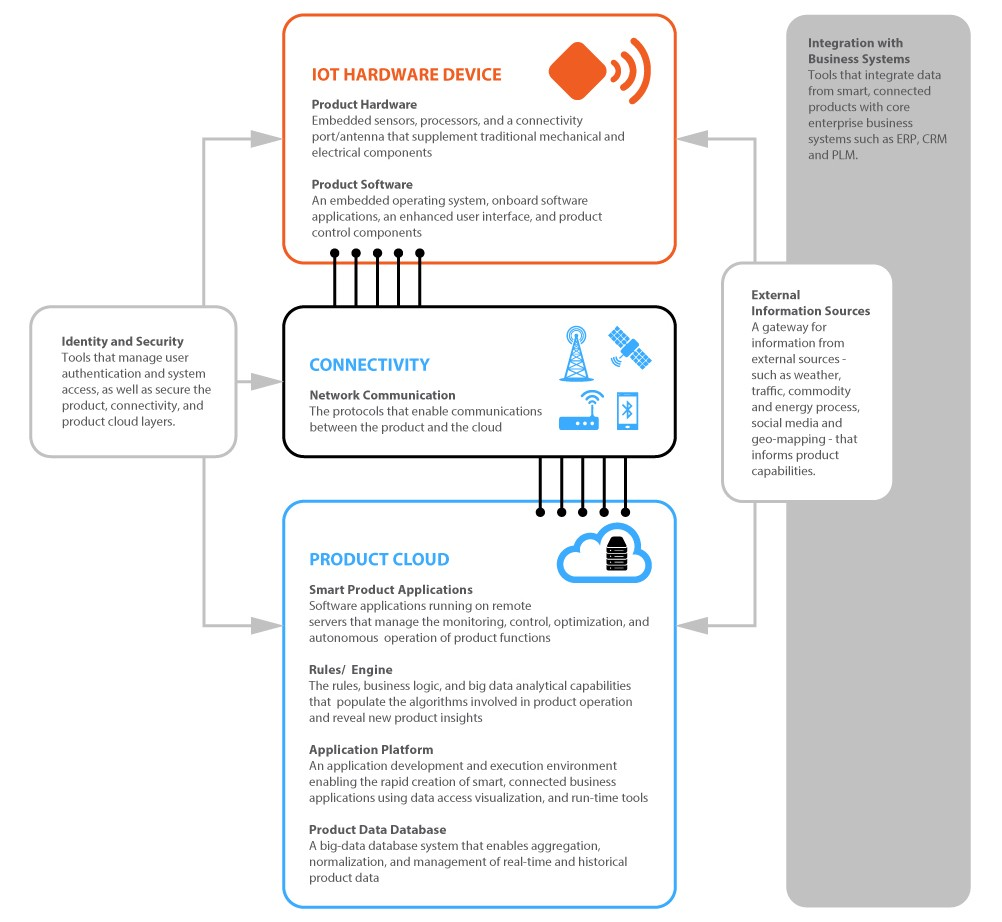
\includegraphics[trim={1cm, 0cm, 0cm, 0cm}, width=18cm, clip]{../../figs/iot_arch.jpeg}
                  \caption{Représentation de l'architecture d'un projet de réseau intélligent.}
                  \label{fig:arch}
            \end{figure}
      \item Citez en donnant les fonctions de chaque couches de l'architecture des réseaux intélligents.
            \begin{itemize}
                  \item  Composant hardware : le dispositif physique qui interagit avec l’environnement.
                  \item Connectivité : le lien entre votre appareil et le cloud
                  \item produits du cloud : serveurs qui prennent des données, les traitent, les
                        stockent dans des bases de données, donnent des commandes, effectuent
                        des analyses, servent les données de manière utile à tous les différents
                        acteurs.
            \end{itemize}
      \item Citez 05 (cinq) protocoles des réseaux intélligents.
            \begin{itemize}
                  \item Bluetooth
                  \item LoRaWAN
                  \item RFID/NFC
                  \item WiFi
                  \item 6LoWPAN
            \end{itemize}
      \item Quelle est la couche de l'architecture des réseaux intélligents qui interagit directement avec les processus industriels ?
            \begin{itemize}
                  \item Couche Hardware ou matériel.
                  \item Cette interaction se fait à travers de capteurs et actionneurs.
            \end{itemize}
      \item Donnez la différence entre un réseaux dit "non intélligent" et un réseaux intélligent.
            \begin{itemize}
                  \item{Les réseaux intelligents sont des réseaux matériels de distributions de fluides (électricité, eau, gaz, pétrole...), et/ou d'information (télécommunications) qui ont été « augmentés » (rendus intelligents) par des systèmes informatiques, capteurs, interfaces informatiques et électromécaniques leur donnant des capacités d'échange bidirectionnel et parfois une certaine capacité d'autonomie en matières de calcul et gestion de flux et traitement d'information.}
            \end{itemize}
\end{enumerate}
La figure \ref{fig:iiot} montre le chef mécanicien vérifiant et contrôlant des robots robots d'automatisation des bras dans l'industrie intelligente d'usine sur le logiciel de système de surveillance en temps réel.

\begin{enumerate}
    \item Donnez trois (03) protocoles réseaux adaptés dans la mise en place de ce réseau intélligent industriel (voir figure \ref{fig:iiot}).
          \begin{itemize}
              \item Wifi
              \item LoRaWan
              \item GSM/GPRS
          \end{itemize}
    \item Donnez les élements de chaque couche de l'architecture d'un réseau intélligent se trouvant sur la figure \ref{fig:iiot}.
          \begin{itemize}
              \item Couche Hardware: représentée par les robots et capteur connectés au serveur central.
              \item Couche de connectivité: représentée par les protocoles réseaux (LoRaWan, Wifi, GSM/GPRS, etc.)
              \item Couche du cloud: représentée par l'ordinateur central du mécanicien chef.
          \end{itemize}
    \item Donnez deux (02) avantages de ce réseau sur une industrie.
          \begin{enumerate}
              \item Une augmentation de production
              \item Favorise une meilleure collaboration entre les employés.
              \item Facilite l'échange et le partage d’information au sein de l'industrie.
              \item Garantie une sécurité des employés car le contrôle se faits à distance.
          \end{enumerate}
    \item Donnez deux (03) tâches à éffectuer afin d'éviter l'attaque des robots réseau sur les employés de cette l'industrie.
          \begin{enumerate}
              \item Rendre le matériel (robots, capteurs, etc.) inviolable.
              \item Utilisation d'une l’authentification forte.
              \item Utiliser un cryptage fort et des protocoles sécurisés.
              \item Diviser les réseaux en segments.
          \end{enumerate}
\end{enumerate}

\begin{figure}[!ht]
    \centering
    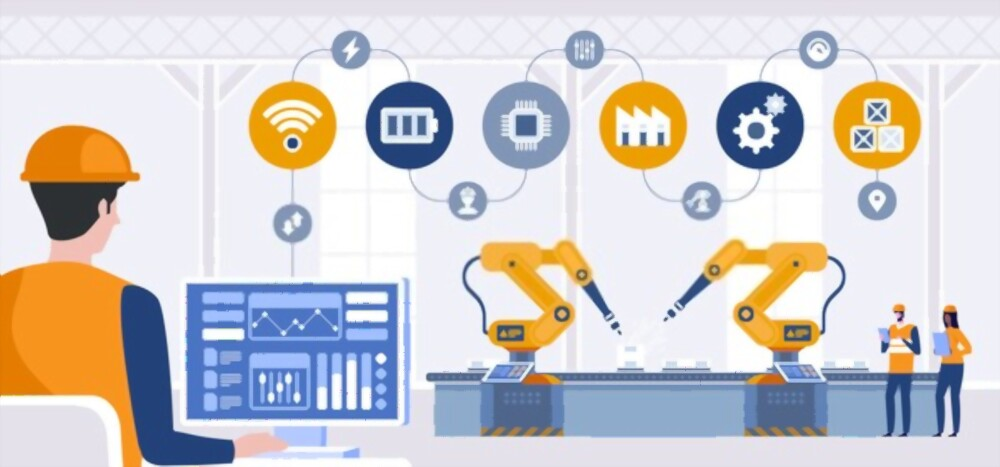
\includegraphics[scale=1.4]{../../figs/industrial_inttelings.jpg}
    \caption{Le chef mécanicien vérifie et contrôle des robots, robots d'automatisation à bras dans l'industrie intelligente d'usine sur le logiciel de système de surveillance en temps réel.}
    \label{fig:iiot}
\end{figure}